% !TEX encoding = UTF-8 Unicode
% !TEX TS-program = xelatex
\begin{QUESTIONS}
	\setcounter{enumi}{8}
\begin{QUESTION}
    \begin{QBODY}	設$m,n$為小於或等於4的相異正整數且$a,b$為非零實數。已知函數$f(x)=a{{x}^{m}}$與函數$g(x)=b{{x}^{n}}$的圖形恰有3個相異交點,請選出可能的選項。
        \begin{QOPS}
        \QOP $m,n$皆為偶數且$a,b$同號 
        \QOP $m,n$皆為偶數且$a,b$異號
        \QOP $m,n$皆為奇數且$a,b$同號
        \QOP $m,n$皆為奇數且$a,b$異號
        \QOP $m,n$為一奇一偶
        \end{QOPS}
    \end{QBODY}
    \begin{QFROMS}
    \end{QFROMS}
    \begin{QTAGS}
    \end{QTAGS}
    \begin{QANS}
        (1)(3)
    \end{QANS}
    \begin{QSOL}
    \end{QSOL}
    \begin{QEMPTYSPACE}
    \end{QEMPTYSPACE}
\end{QUESTION}
\begin{QUESTION}
    \begin{QBODY}
        設$\Gamma $為坐標平面上的圓,點$(0,0)$在$\Gamma $的外部且點$(2,6)$在$\Gamma $的內部。請選出正確的選項。
        \begin{QOPS}
        \QOP $\Gamma $的圓心不可能在第二象限
        \QOP $\Gamma $的圓心可能在第三象限且此時$\Gamma $的半徑必定大於10
        \QOP $\Gamma $的圓心可能在第一象限且此時$\Gamma $的半徑必定小於10
        \QOP $\Gamma $的圓心可能在$x$軸上且此時圓心的$x$坐標必定小於10
        \QOP $\Gamma $的圓心可能在第四象限且此時$\Gamma $的半徑必定大於10
        \end{QOPS}
    \end{QBODY}
    \begin{QFROMS}
    \end{QFROMS}
    \begin{QTAGS}
    \end{QTAGS}
    \begin{QANS}
        (5)
    \end{QANS}
    \begin{QSOL}
    \end{QSOL}
    \begin{QEMPTYSPACE}
    \end{QEMPTYSPACE}
\end{QUESTION}
\begin{QUESTION}
    \begin{QBODY}
        坐標空間中有三直線${{L}_{1}}:\dfrac{x-1}{2}=\dfrac{y+1}{2}=\dfrac{z}{1},{{L}_{2}}:\left\{ \begin{aligned}
        & x-2y+2z=-4 \\ 
        & x+y-4z=5 \\ 
        \end{aligned} \right.,{{L}_{3}}:\left\{ \begin{aligned}
        & x=-t \\ 
        & y=-2-t \\ 
        & z=4+4t \\ 
        \end{aligned} \right.$,$t$為實數。請選出正確的選項。
        \begin{QOPS}
            \QOP ${{L}_{1}}$與${{L}_{2}}$的方向向量互相垂直
            \QOP ${{L}_{1}}$與${{L}_{3}}$的方向向量互相垂直
            \QOP 有一個平面同時包含${{L}_{1}}$與${{L}_{2}}$
            \QOP 有一個平面同時包含${{L}_{1}}$與${{L}_{3}}$
            \QOP 有一個平面同時包含${{L}_{2}}$與${{L}_{3}}$
        \end{QOPS}
    \end{QBODY}
    \begin{QFROMS}
    \end{QFROMS}
    \begin{QTAGS}
    \end{QTAGS}
    \begin{QANS}
        (2)(3)(4)
    \end{QANS}
    \begin{QSOL}
    \end{QSOL}
    \begin{QEMPTYSPACE}
    \end{QEMPTYSPACE}
\end{QUESTION}
\begin{QUESTION}
    \begin{QBODY}
        設最近數學家發現一種新的可以無縫密舖平面的凸五邊形$ABCDE$,其示意圖如下。關於這五邊形,請選出正確的選項。
        
        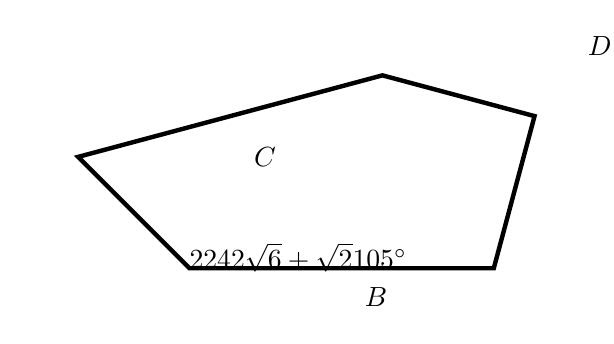
\begin{tikzpicture}[scale=1.0]
        
        \coordinate (B) at (0,0);
        \coordinate (A) at (0:{sqrt(6)+sqrt(2)});
        \path (A) ++(75:2) coordinate (E);
        \path (E) ++(165:2) coordinate (D);
        \coordinate (C) at (135:2);
        
        
        \draw[ultra thick] (A) -- (B)--(C)--(D)--(E) --cycle;
        \tkzLabelSegment[midway,  right](E,A){$2$};
        \tkzLabelSegment[midway,  above](D,E){$2$};
        \tkzLabelSegment[midway,  above](D,C){$4$};
        \tkzLabelSegment[midway,  below left](C,B){$2$};
        \tkzLabelSegment[midway,  below](B,A){$\sqrt{6}+\sqrt{2}$};
        \tkzMarkRightAngle[size=0.3](D,E,A);
        \tkzMarkAngle[size=0.3](E,A,B);
        \tkzLabelAngle[pos=0.6](E,A,B){$105^\circ$};
        
        \node[label=315:$A$] at (A){};
        \node[label=225:$B$] at (B){};
        \node[label=180:$C$] at (C){};
        \node[label=90:$D$] at (D){};
        \node[label=45:$E$] at (E){};
        \end{tikzpicture}
        \begin{QOPS}
        \QOP $\overline{AD}=2\sqrt[{}]{2}$
        \QOP $\angle DAB=45{}^\circ $
        \QOP $\overline{BD}=2\sqrt[{}]{6}$
        \QOP $\angle ABD=45{}^\circ $
        \QOP $BCD$的面積為$2\sqrt[{}]{2}$
        \end{QOPS}
    \end{QBODY}
    \begin{QFROMS}
    \end{QFROMS}
    \begin{QTAGS}
    \end{QTAGS}
    \begin{QANS}
        (1)(4)
    \end{QANS}
    \begin{QSOL}
    \end{QSOL}
    \begin{QEMPTYSPACE}
    \end{QEMPTYSPACE}
\end{QUESTION}
\begin{QUESTION}
    \begin{QBODY}
        某班級50位學生,段考國文、英文、數學及格的人數分別為45、39、34人,且英文及格的學生國文也都及格。現假設數學和英文皆及格的有$x$人,數學及格但英文不及格的有$y$人。請選出正確的選項。
        \begin{QOPS}
            \QOP $x+y=39$
            \QOP $y\le 11$
            \QOP 三科中至少有一科不及格的學生有$39-x+y$人
            \QOP 三科中至少有一科不及格的學生最少有11人
            \QOP 三科中至少有一科不及格的學生最多有27人
        \end{QOPS}
    \end{QBODY}
    \begin{QFROMS}
    \end{QFROMS}
    \begin{QTAGS}
    \end{QTAGS}
    \begin{QANS}
        (2)(5)
    \end{QANS}
    \begin{QSOL}
        \begin{QSTEPS}
            \QSTEP{ 令全班為集合$U$,國文、數學、英文,及格的集合分別為 $C,M,E$ \\
                    可得:$n(C) = 45, n(M) = 34 , n(E) = 39$}
            \QSTEP{ $x+y = n (M \cap E) + n (M \cap \overline{E}) = n(M) = 34$,則 (1) 錯誤}
            \QSTEP{ $n(\bar{E}) = 50 -39 =11 \ge n (M \cap \bar{E}) \Rightarrow y \le 11$,則 (2) 正確}
            \QSTEP{ 由以上兩步驟可得 $23 \le x\le 34$}
            \QSTEP{ 至少一科不及格 $= n(\text{全}) - n (C\cap M\cap E) = 50-x$,\\
                    可得 $16 \le \text{至少一科不及格} \le 27$}
        \end{QSTEPS}
        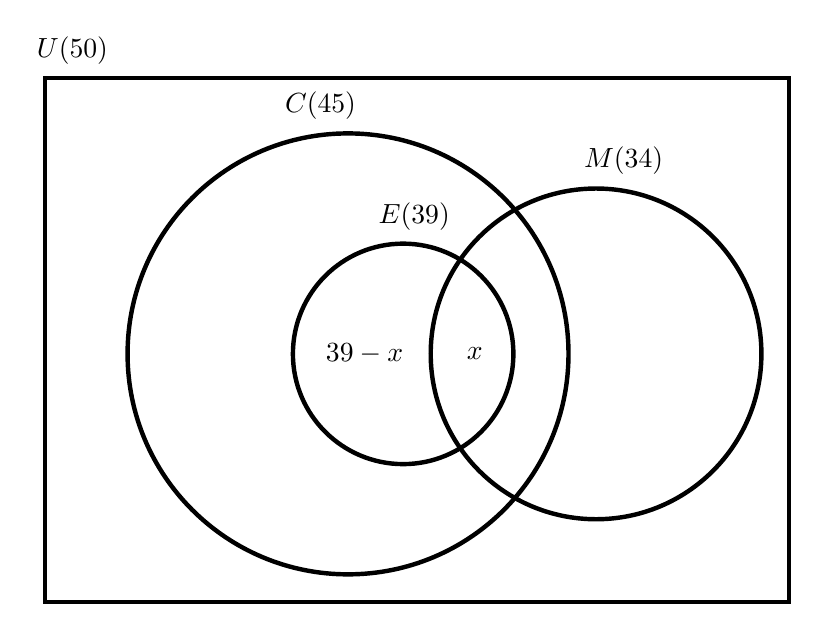
\begin{tikzpicture}[scale=0.7]
            \draw[ultra thick]  (-6.5,6) circle (2);
            \draw[ultra thick]  (-7.5,6) node (v1) {} ellipse (4 and 4);
            
            
            \draw[ultra thick]  (-3,6) node (v2) {} circle (3);
            
            \draw[ultra thick]  (-13,11) rectangle (0.5,1.5);
            
            \node at (-12.5,11.5) {$U(50)$};
            \node at (-8,10.5) {$C(45)$};
            
            \node at (-5.2,6) {$x$};
            
            \node at (-7.2,6) {$39-x$};
            \node at (-6.3,8.5) {$E(39)$};
            
            \node at (-2.5,9.5) {$M(34)$};
    \end{tikzpicture}
    \end{QSOL}
    \begin{QEMPTYSPACE}
    \end{QEMPTYSPACE}
\end{QUESTION}
\begin{QUESTION}
    \begin{QBODY}
        空間中有一四面體$ABCD$。假設$\lvec{AD}$分別與$\lvec{AB}$和$\lvec{AC}$垂直,請選出正確的選項。
        \begin{QOPS}
            \QOP $\lvec{DB}\cdot\lvec{DC} ={{\overline{DA}}^{2}}- \lvec{AB}\cdot \lvec{AC}$
            \QOP 若$\angle BAC$是直角,則$\angle BDC$是直角
            \QOP 若$\angle BAC$是銳角,則$\angle BDC$是銳角
            \QOP 若$\angle BAC$是鈍角,則$\angle BDC$是鈍角
            \QOP 若$\overline{AB}<\overline{DA}$且$\overline{AC}<\overline{DA}$,則$\angle BDC$是銳角
        \end{QOPS}
    \end{QBODY}
    \begin{QFROMS}
    \end{QFROMS}
    \begin{QTAGS}
    \end{QTAGS}
    \begin{QANS}
        (3)(5)
    \end{QANS}
    \begin{QSOL}
    \end{QSOL}
    \begin{QEMPTYSPACE}
    \end{QEMPTYSPACE}
\end{QUESTION}
\end{QUESTIONS}